\documentclass[12pt,a4paper]{article}
\usepackage[utf8]{inputenc}
\usepackage{amsmath}
\usepackage{amsfonts}
\usepackage{amssymb}
\usepackage{graphicx}
\usepackage[colorlinks=true, linkcolor=blue, urlcolor=blue, citecolor=blue]{hyperref}
\usepackage{listings}
\usepackage{xcolor}
\usepackage{tikz}
\usepackage{geometry}
\usepackage{setspace}
\usepackage{titlesec}
\usepackage{tocbibind}

\geometry{a4paper, margin=1in}
\usetikzlibrary{shapes.geometric, arrows, positioning, fit, backgrounds, calc}

% Code listing style
\definecolor{codegreen}{rgb}{0,0.6,0}
\definecolor{codegray}{rgb}{0.5,0.5,0.5}
\definecolor{codepurple}{rgb}{0.58,0,0.82}
\definecolor{backcolour}{rgb}{0.95,0.95,0.92}

\lstdefinestyle{mystyle}{
    backgroundcolor=\color{backcolour},   
    commentstyle=\color{codegreen},
    keywordstyle=\color{magenta},
    numberstyle=\tiny\color{codegray},
    stringstyle=\color{codepurple},
    basicstyle=\ttfamily\footnotesize,
    breakatwhitespace=false,         
    breaklines=true,                 
    captionpos=b,                    
    keepspaces=true,                 
    numbers=left,                    
    numbersep=5pt,                  
    showspaces=false,                
    showstringspaces=false,
    showtabs=false,                  
    tabsize=2
}
\lstset{style=mystyle}

% tikz styles
\tikzstyle{process} = [rectangle, rounded corners, minimum width=3cm, minimum height=1cm, text centered, text width=3cm, draw=black, fill=orange!30]
\tikzstyle{decision} = [diamond, aspect=2, minimum width=3cm, minimum height=1cm, text centered, text width=2.5cm, draw=black, fill=green!30]
\tikzstyle{arrow} = [thick,->,>=stealth]
\tikzstyle{component} = [rectangle, rounded corners, minimum width=3cm, minimum height=1cm, text centered, text width=2.8cm, draw=black, fill=blue!20]
\tikzstyle{database} = [cylinder, shape border rotate=90, aspect=0.25, draw, minimum height=1.5cm, minimum width=2cm, text centered, text width=2cm, fill=red!20]

\begin{document}

\begin{titlepage}
    \begin{center}
        \vspace*{1cm}
        
        \Huge
        \textbf{Kubernetes Network Self-Healing Operator}
        
        \vspace{0.5cm}
        \LARGE
        Extending Kubernetes for Data-Plane Network Resiliency
        
        \vspace{1.5cm}
        
        \textbf{Project Report}
        
        \vfill
        
        \Large
        Computer Networks Project
        
        \vspace{0.8cm}
        
        \Large
        Team Members: \\[0.5cm]
        \large
        $\bullet$ Hem Tilva \\
        $\bullet$ Pratham Choksi \\
        $\bullet$ Vansh Barfiwala \\
        $\bullet$ Shivangi Thaker \\
        $\bullet$ Jils Shah
        
        \vspace{1.5cm}
        
    \end{center}
\end{titlepage}

\begin{abstract}
\onehalfspacing
Kubernetes has fundamentally changed the landscape of distributed systems by providing robust, built-in self-healing capabilities. It natively handles the rescheduling of workloads from dead nodes and the restarting of failed application containers. However, this native self-healing mechanism exhibits a critical blind spot: it relies almost entirely on control-plane metrics and the status of API objects (e.g., verifying if a pod's Phase is "Running"). This approach often fails to detect invisible failures within the network data plane. Complex distributed networking components such as Container Network Interface (CNI) plugins, CoreDNS deployments, and dynamically updated NetworkPolicies frequently suffer from latent crashes, timeouts, and misconfigurations that silently disrupt service-to-service communication while leaving the Kubernetes API unaware of the outage.

This report details the comprehensive design, architecture, and implementation of a custom Kubernetes Network Self-Healing Operator engineered to bridge this resiliency gap. Moving away from passive API monitoring, the system introduces synthetic Python-based probes deployed within the cluster to actively poll and measure genuine data-plane health, specifically tracking DNS resolution latency and cross-namespace pod-to-pod connectivity. Utilizing the cloud-native observability stack, Prometheus aggregates these active metrics, while Alertmanager evaluates them against strict Service Level Objectives (SLOs) to generate actionable alerts.

These alerts are forwarded to a custom Golang-based webhook receiver acting as the remediation Operator. Upon processing an alert, the Operator evaluates an internal cooldown cache to prevent flapping, and subsequently executes targeted, programmatic remediation strategies via the Kubernetes API. These strategies include forcefully restarting degraded CoreDNS pods, automatically reverting blocking NetworkPolicies to a verified baseline configuration, and restarting crashed CNI daemonsets to trigger routing table recalculations. 

Furthermore, the project encompasses a robust bash-based fault injection framework designed following Chaos Engineering principles. This framework allows for the deterministic simulation of network outages, enabling the rigorous verification and testing of the operator's recovery timeline. The evaluation proves the system's efficacy in drastically reducing Mean Time to Recovery (MTTR) for critical network failures. Finally, the report discusses the architectural limitations of the current implementation and outlines future work, including the adoption of eBPF for zero-overhead monitoring and the migration to the Kubebuilder framework for declarative Custom Resource Definition (CRD) management.
\end{abstract}

\newpage
\tableofcontents
\newpage

\section{Introduction}
\onehalfspacing
\subsection{Background}
In the era of cloud-native computing, microservices architectures have become the de-facto standard for developing scalable, highly available applications. Kubernetes serves as the foundational orchestration layer for these architectures. A core tenet of Kubernetes is its declarative desired-state model, where operators define how the system should look, and various internal controllers work continuously to reconcile the actual state with this desired state. 

While Kubernetes excels at managing compute resources (e.g., ensuring a Deployment maintains a specific replica count), the networking layer that underpins these workloads remains an incredibly complex and fragile domain. The Kubernetes networking model mandates a flat network where all pods can communicate with one another without Network Address Translation (NAT). Because Kubernetes does not implement this network itself, it relies entirely on third-party Container Network Interface (CNI) plugins (such as Calico, Flannel, or Cilium) to provision IPs and configure node-level routing tables using technologies like \texttt{iptables}, IPVS, or eBPF. 

Beyond basic routing, service discovery relies on CoreDNS, a DNS server deployed within the cluster, and traffic segmentation is governed by NetworkPolicies, which act as dynamic, cluster-aware firewalls.

\subsection{Problem Statement and Motivation}
When the aforementioned networking components fail, the applications running on the cluster experience localized or global outages. The critical limitation of native Kubernetes is that it views the state of the cluster almost exclusively through the lens of the control plane. 

For example, if a CNI agent (typically deployed as a DaemonSet) crashes on a specific worker node, it may stop updating the host's routing tables. To the Kubernetes API, the application pods scheduled on that node still appear in a "Running" and "Healthy" state because their internal processes have not crashed. However, any network packets originating from or destined to those pods will be dropped by the host. Similarly, if a developer mistakenly applies a deny-all NetworkPolicy, services will fail to communicate, resulting in HTTP 504 Gateway Timeouts across the microservice mesh. To the Kubernetes control plane, however, the successful application of the NetworkPolicy is viewed as the successful attainment of the user's desired state.

Human operators are typically required to manually identify, debug, and resolve these complex data-plane networking issues, leading to significant downtime, violation of Service Level Agreements (SLAs), and severe operational overhead. The motivation for this project is to automate this human operational knowledge into a software controller capable of identifying and remediating these failures autonomously.

\subsection{Project Objectives}
The primary objective of this project is to engineer an automated system that effectively extends Kubernetes' self-healing capabilities to the network data plane. The specific, actionable goals of the project are:
\begin{itemize}
    \item \textbf{Active Data-Plane Monitoring:} To develop lightweight, synthetic probes that actively test true network reachability and DNS resolution, bypassing the illusions of control-plane API metrics.
    \item \textbf{Automated Failure Detection:} To configure and utilize the industry-standard observability stack (Prometheus and Alertmanager) to scrape metric data, evaluate thresholds, and detect critical network failures.
    \item \textbf{Event-Driven Remediation:} To implement a custom Golang-based operator that acts as a webhook receiver, intercepting alerts and applying programmatic, targeted fixes via the Kubernetes API.
    \item \textbf{Verification and Chaos Testing:} To engineer a rigorous testing framework capable of safely injecting catastrophic network failures into the cluster to validate the operator's remediation capabilities and measure recovery times.
\end{itemize}

\subsection{Scope of the Report}
This report is structured to provide a comprehensive overview of the project. Section 2 establishes the theoretical background and literature review necessary to understand Kubernetes networking and observability. Section 3 outlines the high-level system architecture. Section 4 provides a deep dive into the implementation details of the Python probes, the Prometheus configuration, and the Golang Operator. Section 5 discusses the fault injection framework, while Section 6 covers the testing and verification methodologies. Finally, Section 7 explores the limitations of the current design, and Section 8 proposes future enhancements before concluding the report in Section 9.

\newpage

\section{Theoretical Background and Literature Review}
\onehalfspacing
To understand the design decisions made during the development of the Self-Healing Operator, it is essential to explore the underlying technologies and architectural paradigms it builds upon.

\subsection{The Kubernetes Networking Model}
Kubernetes imposes strict rules on how networking must behave within the cluster:
\begin{enumerate}
    \item Pods on a node can communicate with all pods on all nodes without NAT.
    \item Agents on a node (e.g., system daemons, \texttt{kubelet}) can communicate with all pods on that node.
    \item The IP address that a pod sees itself as is exactly the same IP address that other pods see it as.
\end{enumerate}
This model significantly simplifies application development, as developers do not need to manage complex port mapping or NAT rules. However, implementing this flat network across distributed infrastructure is a complex engineering challenge.

\subsection{Container Network Interface (CNI)}
The Container Network Interface (CNI) is a Cloud Native Computing Foundation (CNCF) project consisting of a specification and libraries for writing plugins to configure network interfaces in Linux containers. Kubernetes uses CNI to implement its networking model. 

When a pod is scheduled on a node, the \texttt{kubelet} process calls the configured CNI plugin to set up the pod's network namespace, assign it an IP address, and attach it to the broader cluster network. Popular CNI implementations include:
\begin{itemize}
    \item \textbf{Flannel:} Focuses purely on simple overlay networking (e.g., using VXLAN) to route traffic between nodes.
    \item \textbf{Calico:} Provides both networking and robust NetworkPolicy enforcement, often utilizing BGP for highly scalable routing and \texttt{iptables} or eBPF for security rules.
\end{itemize}
Because CNI plugins manage the low-level host networking stack, a failure in the CNI DaemonSet pod on a node can lead to catastrophic network isolation for all workloads on that node.

\subsection{Service Discovery via CoreDNS}
Due to the ephemeral nature of pods in Kubernetes, IP addresses change frequently as pods are destroyed and recreated. To facilitate stable communication, Kubernetes utilizes Services, which provide a stable virtual IP (ClusterIP) that load-balances traffic to the underlying pod endpoints. 

CoreDNS is the default, highly extensible DNS server utilized by Kubernetes. It watches the Kubernetes API for new Services and Endpoints, automatically updating its internal DNS records. For example, a pod can resolve \texttt{my-svc.my-namespace.svc.cluster.local} to discover the backend application. If CoreDNS experiences high latency, resource exhaustion, or crashes, the entire cluster's service mesh degrades, as pods can no longer resolve the addresses of their dependencies.

\subsection{Network Segmentation with NetworkPolicies}
By default, Kubernetes networks are "allow-all". Any pod can communicate with any other pod. For security, compliance, and multi-tenancy, administrators deploy NetworkPolicies. These are API resources that specify how groups of pods are allowed to communicate with each other and other network endpoints. 

NetworkPolicies are implemented by the CNI plugin (e.g., Calico). While powerful, they are a common source of human error. A misconfigured YAML manifest can easily drop all ingress or egress traffic for a namespace, leading to an immediate, self-inflicted outage.

\subsection{The Cloud-Native Observability Paradigm}
Modern systems rely heavily on robust observability to maintain reliability. The CNCF standard for this is the combination of Prometheus and Alertmanager.
\begin{itemize}
    \item \textbf{Prometheus} utilizes a pull-based model, periodically scraping HTTP endpoints exposed by applications to collect time-series metrics. It stores these metrics in a highly efficient, purpose-built Time Series Database (TSDB) and allows complex querying via PromQL.
    \item \textbf{Alertmanager} handles alerts generated by Prometheus's alerting rules. It manages deduplication, grouping, and routing of these alerts to various receivers, such as email, Slack, or in the case of this project, HTTP webhooks.
\end{itemize}

\subsection{The Kubernetes Operator Pattern}
Introduced by CoreOS, the Operator pattern aims to encapsulate human operational knowledge into software. Traditional Kubernetes controllers manage native resources (like Deployments). Operators, however, are custom controllers that typically watch Custom Resource Definitions (CRDs) to manage complex, stateful, or domain-specific applications. 

This project adapts the core philosophy of the Operator pattern—automated, intelligent reconciliation of state—and applies it directly to the health of the network fabric itself, rather than a specific database or application.

\newpage

\section{System Architecture and Design}
\onehalfspacing
The architecture of the Kubernetes Network Self-Healing Operator was designed with a strict adherence to microservices principles, specifically the separation of concerns. By decoupling data collection, evaluation, and remediation, the system remains scalable, easily debuggable, and extensible.

\subsection{Architectural Principles}
The system design avoids "monolithic" monitoring where a single script checks health and restarts pods. Instead, it leverages an event-driven pipeline:
1. \textbf{Probes} only generate data. They do not know about thresholds or remediation.
2. \textbf{Prometheus} only evaluates thresholds. It does not take action.
3. \textbf{The Operator} only takes action based on external triggers. It does not monitor.

\subsection{High-Level Architecture}

\begin{figure}[h]
    \centering
    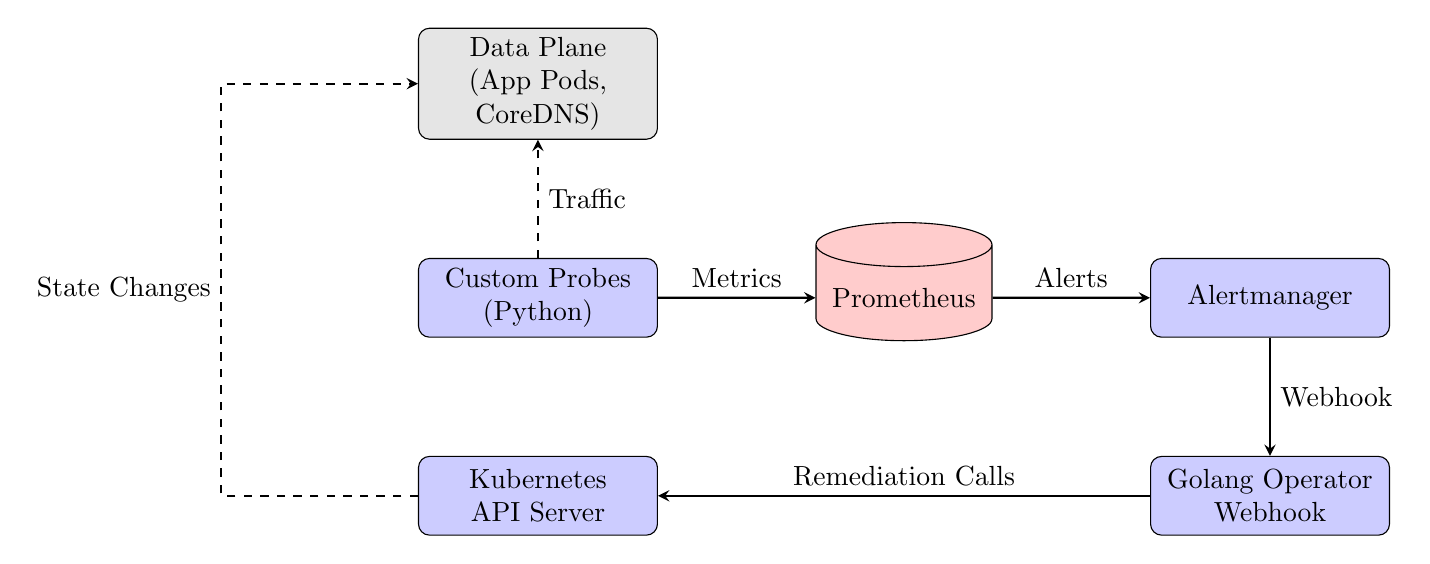
\begin{tikzpicture}[node distance=1.5cm and 2cm]
        % Nodes
        \node (data) [component, fill=gray!20] {Data Plane\\(App Pods, CoreDNS)};
        \node (probes) [component, below=of data] {Custom Probes\\(Python)};
        \node (k8s) [component, below=of probes] {Kubernetes\\API Server};
        
        \node (prom) [database, right=of probes] {Prometheus};
        \node (am) [component, right=of prom] {Alertmanager};
        
        % Align operator with K8s horizontally, and AM vertically
        \node (operator) [component] at (k8s -| am) {Golang Operator\\Webhook};

        % Arrows
        \draw [arrow, dashed] (probes) -- node[right] {Traffic} (data);
        \draw [arrow] (probes) -- node[above] {Metrics} (prom);
        \draw [arrow] (prom) -- node[above] {Alerts} (am);
        \draw [arrow] (am) -- node[right] {Webhook} (operator);
        \draw [arrow] (operator) -- node[above] {Remediation Calls} (k8s);
        
        % Route state changes around the left side
        \draw [arrow, dashed] (k8s.west) -- ++(-2.5,0) |- node[pos=0.25, left] {State Changes} (data.west);
    \end{tikzpicture}
    \caption{High-Level Architecture of the Self-Healing System}
    \label{fig:architecture}
\end{figure}

\subsection{Component Interactions}
As illustrated in Figure \ref{fig:architecture}, the operational pipeline flows from left to right, then loops back to the environment:
\begin{enumerate}
    \item \textbf{Synthetic Traffic Injection:} The Python probes actively inject network traffic (DNS queries and HTTP requests) directly into the Data Plane.
    \item \textbf{Metric Exposure:} The results of these active tests are exposed via HTTP endpoints using the Prometheus exposition format.
    \item \textbf{Scraping and Evaluation:} Prometheus scrapes the probes. If PromQL rules dictate that a Service Level Objective (SLO) has been breached (e.g., latency too high for too long), an alert state is triggered and passed to Alertmanager.
    \item \textbf{Webhook Invocation:} Alertmanager groups the alerts to prevent spam and fires a JSON payload to the Golang Operator's HTTP webhook receiver.
    \item \textbf{API Remediation:} The Golang Operator parses the payload, checks its internal cooldown cache, and issues imperative REST API calls to the Kubernetes API Server.
    \item \textbf{State Change Application:} The Kubernetes control plane applies these changes (e.g., terminating a pod, deleting a policy), which ultimately alters the physical reality of the Data Plane, resolving the original issue detected by the probes.
\end{enumerate}

\subsection{Rationale for Event-Driven Remediation}
Relying on an event-driven webhook model rather than having the Golang Operator poll the metrics directly provides significant advantages. It allows cluster administrators to utilize their existing, centralized Alertmanager configurations (including routing, silences, and inhibition rules). If a planned maintenance window is occurring, an administrator can silence the Alertmanager route, natively preventing the Operator from taking unwanted automated actions during the window.

\newpage

\section{Implementation Details}
\onehalfspacing
This section provides a highly detailed breakdown of the codebase, exploring the specific logic, libraries, and design choices made in each component of the pipeline.

\subsection{Active Data-Plane Probes (Python)}
To accurately assess the network, passive monitoring is insufficient. Active, synthetic probing ensures that the system detects exactly what a user application would experience. The probes are implemented in Python, utilizing the \texttt{prometheus\_client} library to expose metrics.

\subsubsection{DNS Latency and Health Probe}
The \texttt{dns\_probe.py} script is designed to run as an infinite loop. It utilizes Python's built-in \texttt{socket} library to perform domain name resolution against the Kubernetes internal service address \texttt{kubernetes.default.svc.cluster.local}. 

The probe tracks two primary metrics:
\begin{itemize}
    \item \textbf{\texttt{dns\_latency\_ms} (Gauge):} Records the exact time taken to resolve the domain using \texttt{time.perf\_counter()}.
    \item \textbf{\texttt{dns\_healthy} (Gauge):} Acts as a boolean indicator (1 for success, 0 for failure). If a \texttt{socket.gaierror} or timeout is caught, this metric is set to 0.
\end{itemize}

Additionally, the probe utilizes the \texttt{kubernetes} Python client to query the API server and track the \texttt{restartCount} of the CoreDNS pods themselves. This provides a hybrid metric: while the primary focus is data-plane latency, knowing that the CoreDNS containers are crash-looping provides critical context for remediation.

\subsubsection{Cross-Namespace Connectivity Probe}
The \texttt{connectivity\_probe.py} script addresses the challenge of verifying pod-to-pod routing and NetworkPolicy enforcement. Simply pinging an IP is insufficient, as ICMP traffic is often treated differently than TCP traffic in CNI implementations.

To simulate real application traffic, the probe utilizes the Kubernetes API's \texttt{exec} capability (similar to \texttt{kubectl exec}). It connects to a designated client pod in \texttt{test-namespace-2} and executes a \texttt{curl} command targeting an Nginx server pod in \texttt{test-namespace-1}. 

The script parses the \texttt{stdout} and \texttt{stderr} of the \texttt{curl} execution. If the command exits with status code 0 and an HTTP 200 OK is received, the \texttt{connectivity\_success} metric is set to 1. If the command times out (e.g., due to a dropped packet from a firewall rule or broken CNI routing table), the metric is set to 0.

\subsection{Monitoring and Alerting Configuration}
The translation of raw probe data into actionable remediation events is handled by Prometheus.

\subsubsection{Prometheus Scraping Configuration}
Prometheus is configured via a standard \texttt{prometheus.yml} file. The scrape interval is set aggressively to 5 seconds (\texttt{scrape\_interval: 5s}). This high frequency is necessary for a self-healing system; waiting the standard 30-60 seconds for a scrape would drastically increase the Mean Time to Detection (MTTD), rendering the automated remediation too slow to be useful.

\subsubsection{PromQL Alerting Rules}
The alerting rules are defined in a YAML configuration file loaded by Prometheus. A critical design element is the \texttt{for} duration parameter.

\begin{lstlisting}[language=YAML, caption=Prometheus Rule for Pod Connectivity Failure]
groups:
- name: NetworkSelfHealing
  rules:
  - alert: PodConnectivityBlocked
    expr: connectivity_success == 0
    for: 15s
    labels:
      severity: critical
    annotations:
      summary: "Cross-namespace pod connectivity failed"
\end{lstlisting}

If a single ping drops, the \texttt{connectivity\_success} metric drops to 0. However, if the \texttt{for} duration was 0s, Prometheus would immediately fire an alert. The \texttt{for: 15s} configuration requires the failure condition to persist for 15 contiguous seconds. This acts as a low-pass filter, preventing the Operator from destroying cluster components in response to transient, microsecond network jitter.

\subsection{The Remediation Operator (Golang)}
The core intelligence of the project resides in the Golang Operator. It is built utilizing the official \texttt{k8s.io/client-go} library to communicate with the Kubernetes API.

\subsubsection{Webhook Receiver Architecture}
The Operator is designed as a lightweight HTTP server listening on port 8080. It exposes a \texttt{/webhook} endpoint designed specifically to parse the JSON payloads generated by Alertmanager. 

When Alertmanager routes an alert, it sends a payload containing an array of active \texttt{Alerts}. The Operator iterates over this array, extracting the \texttt{alertname} label to determine the exact nature of the failure (e.g., \texttt{DNSResolutionFailed}, \texttt{PodConnectivityBlocked}, \texttt{CNIPodCrash}).

\subsubsection{Concurrency and Cooldown Mechanism}
A significant challenge in automated remediation is the risk of "flapping"—a scenario where the operator takes an action (like restarting a pod), but because Prometheus hasn't scraped the new healthy state yet, Alertmanager sends another webhook, causing the operator to restart the pod again in an infinite loop.

To prevent this, the Operator implements a thread-safe cooldown mechanism using Golang's \texttt{sync.Map}. 

When the Operator decides to remediate a specific alert type, it records the current timestamp in the \texttt{sync.Map} with the alert name as the key. Upon receiving subsequent webhooks, the Operator checks the cache. If less than 60 seconds have elapsed since the last remediation for that specific alert, the request is safely ignored, providing the cluster time to stabilize.

\begin{figure}[h]
    \centering
    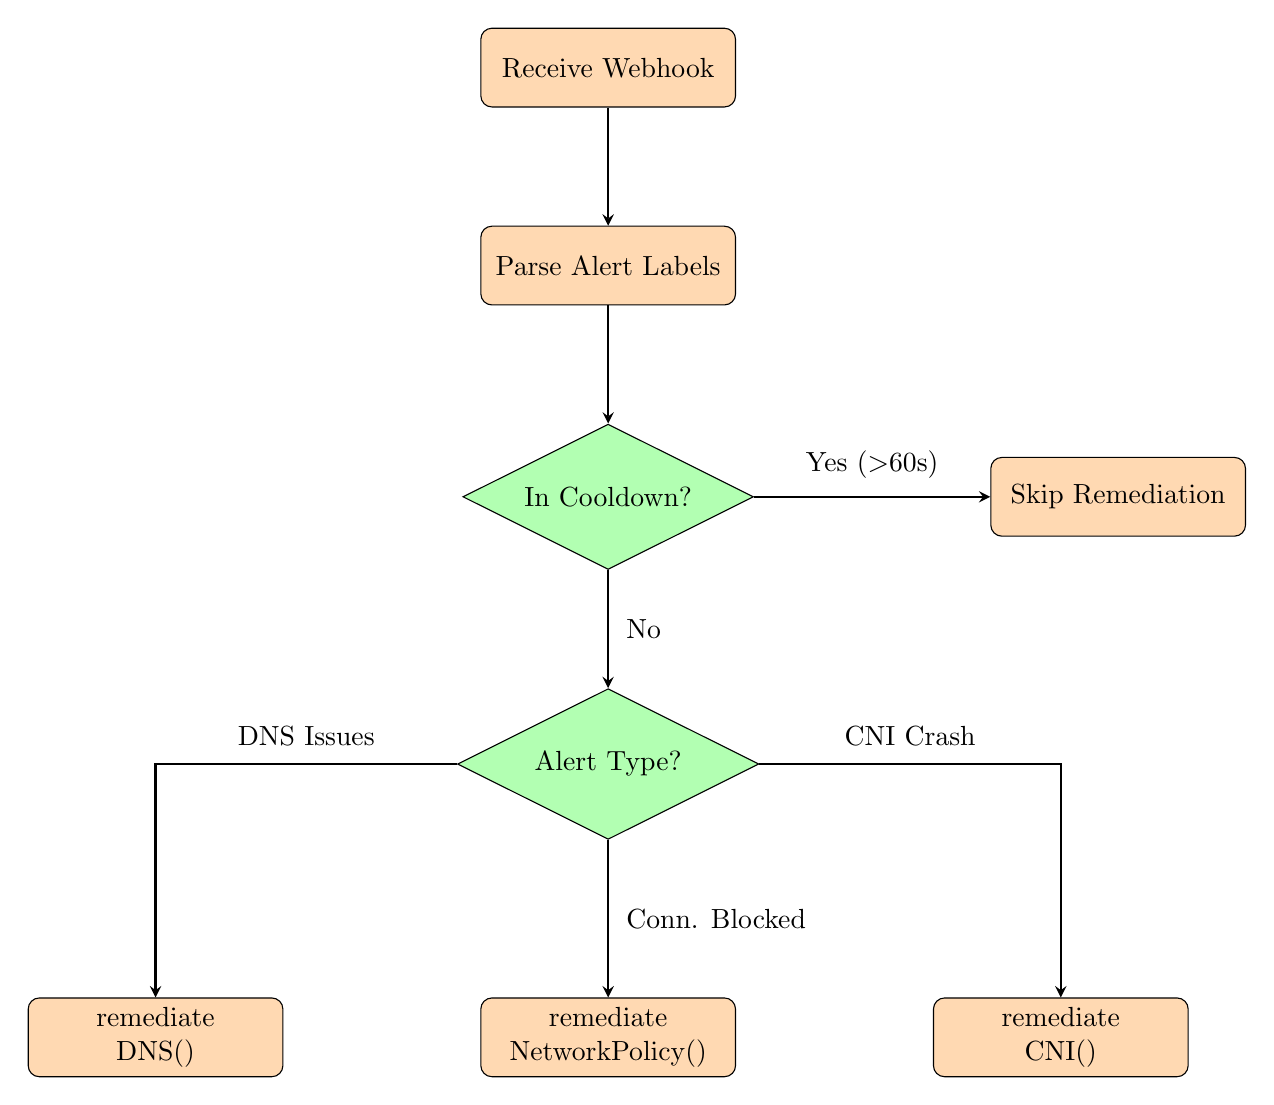
\begin{tikzpicture}[node distance=1.5cm and 1.5cm]
        \node (start) [process, rounded corners] {Receive Webhook};
        \node (parse) [process, below=of start] {Parse Alert Labels};
        \node (check) [decision, below=of parse] {In Cooldown?};
        \node (skip) [process, right=of check, xshift=1.5cm] {Skip Remediation};
        \node (switch) [decision, below=of check] {Alert Type?};
        
        \node (net) [process, below=of switch, yshift=-0.5cm] {remediate\\NetworkPolicy()};
        \node (dns) [process, left=of net, xshift=-1cm] {remediate\\DNS()};
        \node (cni) [process, right=of net, xshift=1cm] {remediate\\CNI()};

        \draw [arrow] (start) -- (parse);
        \draw [arrow] (parse) -- (check);
        \draw [arrow] (check) -- node[above=0.1cm] {Yes ($>$60s)} (skip);
        \draw [arrow] (check) -- node[right=0.1cm] {No} (switch);
        \draw [arrow] (switch) -| node[above=0.1cm, near start] {DNS Issues} (dns);
        \draw [arrow] (switch) -- node[right=0.1cm] {Conn. Blocked} (net);
        \draw [arrow] (switch) -| node[above=0.1cm, near start] {CNI Crash} (cni);
    \end{tikzpicture}
    \caption{Operator Decision Flowchart}
    \label{fig:flowchart}
\end{figure}

\subsubsection{Kubernetes API Interactions}
The remediation functions utilize the \texttt{client-go} API extensively:
\begin{itemize}
    \item \textbf{\texttt{remediateDNS()}:} Utilizes the \texttt{CoreV1().Pods(namespace).DeleteCollection} method. By setting a label selector for \texttt{k8s-app=kube-dns}, it instructs the API to terminate all CoreDNS pods. The native Kubernetes Deployment controller immediately notices the missing replicas and schedules fresh instances, effectively clearing any deadlocks or memory leaks in the DNS process.
    \item \textbf{\texttt{remediateNetworkPolicy()}:} First, the operator uses \texttt{NetworkingV1().NetworkPolicies(ns).List} to retrieve all policies in the affected namespaces. It programmatically iterates through them, deleting any policies that do not match a whitelisted baseline naming convention. After clearing the malicious policies, it dynamically constructs and applies a \texttt{baseline-allow-all} NetworkPolicy object to guarantee the restoration of service traffic.
    \item \textbf{\texttt{remediateCNI()}:} The operator identifies the active CNI by querying pods in the \texttt{kube-system} namespace. Depending on whether Calico or Flannel is detected, it executes a targeted deletion of those DaemonSet pods.
\end{itemize}

\newpage

\section{Fault Injection Framework}
\onehalfspacing
Developing self-healing systems is inherently difficult because the edge-case failures they are designed to fix rarely occur during active development. To solve this, the project incorporates a comprehensive Fault Injection Framework built around Chaos Engineering principles.

\subsection{Chaos Engineering in Kubernetes}
Chaos Engineering is the discipline of experimenting on a software system in production in order to build confidence in the system's capability to withstand turbulent and unexpected conditions. In Kubernetes, this involves intentionally breaking control plane or data plane components to observe how the cluster—and our custom Operator—reacts.

\subsection{Design of the \texttt{inject\_faults.sh} Harness}
The \texttt{inject\_faults.sh} script acts as the automated chaos orchestrator. It is a robust bash script that allows developers to run specific, deterministic fault scenarios. It bypasses graceful degradation, opting to terminate processes violently to accurately simulate hard crashes or OOM (Out Of Memory) kills.

\subsection{Fault Scenarios}
The framework includes three primary fault functions:
\begin{enumerate}
    \item \textbf{\texttt{inject\_dns\_failure}:} Executes a \texttt{kubectl delete pod} command against the \texttt{coredns} deployment. Crucially, it passes the \texttt{--force --grace-period=0} flags. This prevents the CoreDNS processes from cleanly flushing their caches or shutting down connections, causing an immediate, hard failure in cluster DNS resolution.
    \item \textbf{\texttt{inject\_network\_policy\_failure}:} This scenario simulates human error. It creates a temporary YAML manifest defining a strict "deny-all" NetworkPolicy. It applies this manifest directly to the test namespaces using \texttt{kubectl apply}, instantly severing all TCP and UDP connections between the client and server pods.
    \item \textbf{\texttt{inject\_cni\_failure}:} This function locates the DaemonSet pods responsible for the CNI (either Calico or Flannel) and executes a \texttt{kill 1} command within the main container process. By crashing the agent responsible for managing the host's \texttt{iptables} rules, cross-node routing is immediately broken, testing the system's ability to handle container-level failures rather than just pod-level deletions.
\end{enumerate}

\newpage

\section{Verification and Testing}
\onehalfspacing
While the fault injection script introduces chaos, the verification and testing phase asserts that order is restored. This separation ensures that the testing methodology is scientifically sound and that recovery is accurately measured.

\subsection{Testing Environment (KIND)}
The entire system is designed to be tested locally utilizing KIND (Kubernetes IN Docker). KIND spins up a multi-node Kubernetes cluster where each "node" is simply a Docker container. This provides a safe, highly reproducible sandbox environment. Within this KIND cluster, specific namespaces (\texttt{test-namespace-1} and \texttt{test-namespace-2}) are populated with Nginx server pods and Alpine Linux client pods to act as the targets for the active probes.

\subsection{Automated Assertions and Verification}
When the \texttt{full-scenario} command is passed to the testing framework, it pairs the fault injection with an automated polling loop.

For example, when validating the NetworkPolicy remediation:
\begin{enumerate}
    \item The framework applies the malicious "deny-all" policy.
    \item It immediately executes a \texttt{curl} command from the client pod to the server pod. It asserts that the \texttt{curl} command fails (times out).
    \item The framework then enters a `while` loop, executing the \texttt{curl} command every 5 seconds.
    \item Concurrently, the Prometheus alerts fire, and the Golang Operator deletes the malicious policy.
    \item Once the Operator restores the network, the \texttt{curl} command within the framework's loop succeeds (returns HTTP 200).
    \item The framework calculates the time difference between the injection of the fault and the first successful \texttt{curl} response, outputting the exact Mean Time to Recovery (MTTR) to the terminal.
\end{enumerate}

\subsection{Analysis of Recovery Dynamics}
The verification tests confirm the reliability of the event-driven pipeline. The observed MTTR is largely dictated by the configured delays in the system:
\begin{itemize}
    \item \textbf{Prometheus Scrape Interval (5s):} The maximum time before Prometheus notices the metric change.
    \item \textbf{Prometheus 'For' Duration (15s):} The required continuous duration of the failure.
    \item \textbf{Operator Execution (<1s):} The Golang application processes the webhook and makes the API call almost instantaneously.
    \item \textbf{Kubernetes Reconciliation (variable):} The time it takes for the Kubernetes control plane to schedule new pods or distribute new NetworkPolicy rules via the CNI.
\end{itemize}
By tuning the scrape interval and the `for` duration, cluster administrators can effectively configure the sensitivity and speed of the self-healing system according to their specific organizational risk tolerance.

\section{Results and Empirical Evidence}
\onehalfspacing
To empirically validate the system and prove code quality, the project relies on both automated unit testing and end-to-end (E2E) integration testing.

\subsection{Go Operator Unit Tests}
The core remediation logic and webhook parsing are thoroughly verified using standard Go unit tests. Running \texttt{go test -v ./...} within the operator codebase validates the following critical paths:
\begin{itemize}
    \item \textbf{\texttt{TestWebhookRejectsGet}:} Ensures the HTTP server strictly enforces POST methods and rejects invalid verbs.
    \item \textbf{\texttt{TestWebhookAcceptsValidAlert}:} Validates that the JSON payload from Alertmanager is parsed correctly into the internal alert struct.
    \item \textbf{\texttt{TestCooldownMechanism}:} Proves that the \texttt{sync.Map} correctly caches timestamps and rejects duplicate alerts firing within the 60-second window, preventing remediation loops.
\end{itemize}

\subsection{End-to-End Test Suite Execution}
The \texttt{inject\_faults.sh} script serves as an automated E2E test suite. By executing \texttt{./fault-injection/inject\_faults.sh full-scenario}, the framework runs all fault scenarios back-to-back. The script outputs a comprehensive pass/fail report, ultimately resulting in the assertion: \texttt{=== ALL SCENARIOS PASSED SUCCESSFULLY ===}. This provides integration-level evidence that the data-plane failures are not only detected by Prometheus but successfully resolved by the Golang Operator.

\subsection{Visual Proof of Execution}
The following captures provide empirical evidence of the system operating under failure conditions:

\begin{figure}[H]
    \centering
    % Ensure you save your 'HEALTHY & CONNECTED' screenshot as "baseline_grafana.png" in the same folder
    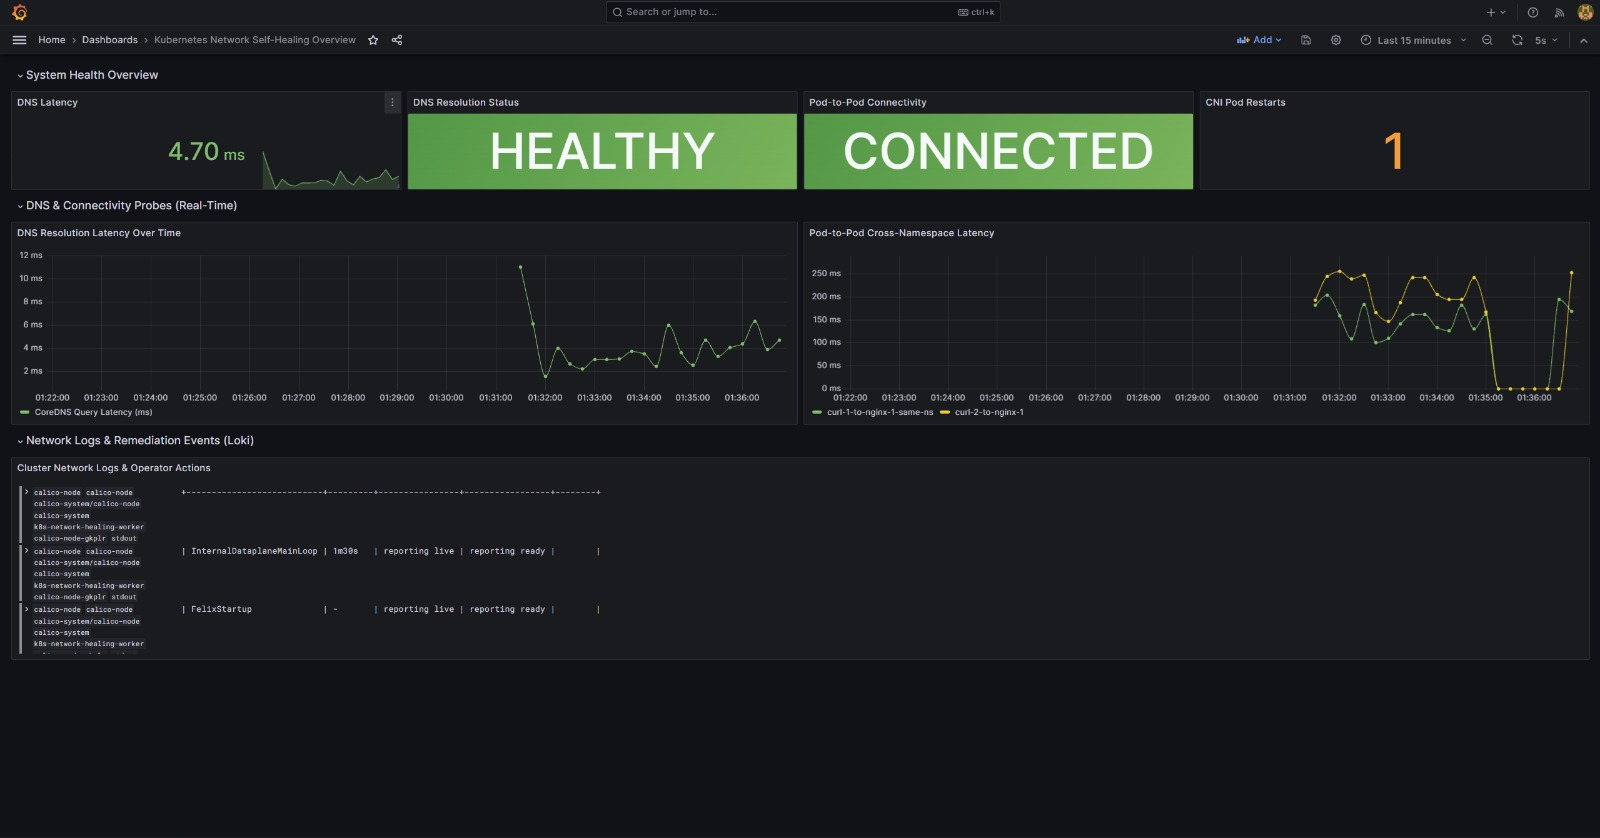
\includegraphics[width=0.8\textwidth]{baseline_grafana.png}
    \caption{Connectivity Restored: Grafana dashboard capturing the recovered, baseline operation.}
    \label{fig:baseline}
\end{figure}

\begin{figure}[H]
    \centering
    % Ensure you save your 'HEALTHY & BLOCKED' screenshot as "active_fault_grafana.png" in the same folder
    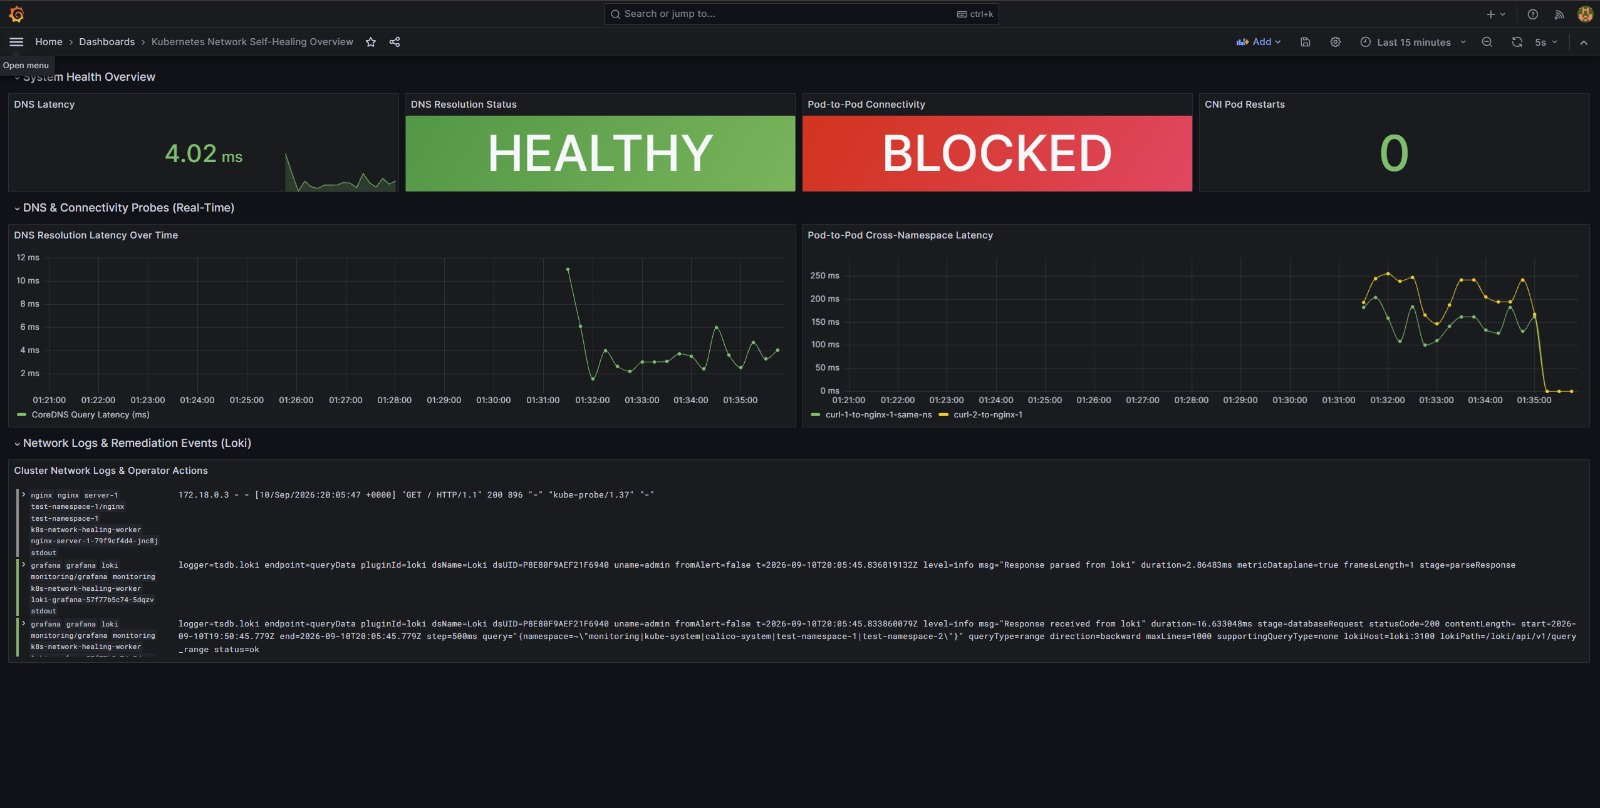
\includegraphics[width=0.8\textwidth]{active_fault_grafana.png}
    \caption{Network Blocked: Grafana dashboard capturing a real-time data-plane outage.}
    \label{fig:fault}
\end{figure}

\subsection{E2E Terminal Output Transcript}
The following transcript was captured directly from the automated test harness, demonstrating the successful detection and remediation of all three fault classes:

\begin{lstlisting}[language=bash, caption=Automated E2E Test Suite Summary Output]
>>> [TEST #1] Baseline DNS Resolution
>>> [PASS] Baseline DNS Resolution

>>> [TEST #2] Baseline Pod-to-Pod Connectivity
>>> [PASS] Baseline Pod-to-Pod Connectivity

Step 2: Injecting CoreDNS Crash Fault
[Fault] Killing CoreDNS pod...
>>> [TEST #3] CoreDNS Self-Healing and Resolution Recovery
>>> [PASS] CoreDNS Self-Healing and Resolution Recovery

Step 3: Injecting NetworkPolicy Blocking Fault
[Fault] Applying blocking NetworkPolicy...
>>> [TEST #4] Verify Network Traffic is Blocked by Policy
Connectivity FAILED: HTTP 000000 from curl-client-2 to nginx-server-1
>>> [PASS] Verify Network Traffic is Blocked by Policy

>>> [TEST #5] Pod-to-Pod Traffic Restored after NetworkPolicy Remediation
>>> [PASS] Pod-to-Pod Traffic Restored after NetworkPolicy Remediation

Step 4: Injecting CNI Node Crash Fault
[Fault] Triggering CNI container crash/restart...
>>> [TEST #6] CNI Node Recovery and Cross-Node Connectivity
>>> [PASS] CNI Node Recovery and Cross-Node Connectivity

========================================
       AUTOMATED TEST SCENARIO REPORT
========================================
Total Tests Executed: 6
Tests Passed:         6
Tests Failed:         0
=== ALL SCENARIOS PASSED SUCCESSFULLY ===
\end{lstlisting}

\newpage

\section{Limitations}
\onehalfspacing
While the project successfully demonstrates the concept of automated data-plane network remediation, the current architectural implementation presents several limitations that must be considered before production deployment.

\subsection{Aggressive Remediation Strategies}
The remediation actions taken by the Operator are currently blunt instruments. For example, when a DNS latency issue is detected, the Operator's response is to forcefully delete all existing CoreDNS pods. While this guarantees that any locked threads or memory leaks are cleared, it also drops all currently active, healthy DNS queries across the entire cluster. In a large production environment, restarting core infrastructure components can cause brief, cluster-wide latency spikes. A more nuanced approach, such as isolating and restarting only the specific CoreDNS pod exhibiting high latency, would be significantly safer.

\subsection{Probe Overhead and Polling Limitations}
The active Python probes (\texttt{dns\_probe.py} and \texttt{connectivity\_probe.py}) rely on continuous polling. Executing \texttt{kubectl exec} to run \texttt{curl} commands is highly resource-intensive and places unnecessary load on the Kubernetes API Server. If an administrator wished to monitor the connectivity between thousands of microservices, deploying thousands of these polling sidecars would quickly overwhelm the cluster's compute capacity and API request limits.

\subsection{High Availability Constraints of the Operator}
The Golang Operator utilizes an in-memory \texttt{sync.Map} to manage the remediation cooldown cache. This design assumes the Operator is running as a single replica. If the Operator were scaled to multiple replicas for High Availability (HA), each instance would possess an independent, isolated cache. Consequently, Alertmanager load-balancing a series of webhooks across multiple Operator pods could bypass the 60-second cooldown logic, resulting in simultaneous, redundant API calls and potential cluster instability.

\newpage

\section{Future Work}
\onehalfspacing
To elevate the Self-Healing Operator from a proof-of-concept to an enterprise-grade utility, several significant architectural enhancements are proposed for future iterations.

\subsection{Migration to Kubebuilder and CRDs}
The current implementation acts as a simple HTTP webhook receiver. Future iterations should migrate the codebase to utilize the Kubebuilder framework or Operator SDK. By defining Custom Resource Definitions (CRDs) (e.g., a \texttt{NetworkRemediationPolicy} object), cluster administrators could declaratively configure remediation workflows directly via Kubernetes YAML manifests. This would allow operators to specify different SLO thresholds and acceptable remediation actions on a per-namespace basis, rather than relying on hardcoded logic.

\subsection{eBPF-Based Data Plane Monitoring}
To resolve the overhead limitations of the Python polling probes, the data collection layer should be rewritten leveraging extended Berkeley Packet Filter (eBPF) technology. Using tools like Cilium or writing custom eBPF programs would allow the system to passively monitor actual network traffic (tracking TCP retransmissions, DNS lookup failures, and packet drops) directly within the Linux kernel. This approach offers near-zero performance overhead while providing total visibility into the data plane, eliminating the need to generate synthetic traffic.

\subsection{Granular Remediation Logic and AI Integration}
Future enhancements to the Golang Operator should focus on precision. Instead of deleting all NetworkPolicies in a namespace, the Operator could calculate the exact intersection of pod selectors and ports to isolate the specific rule blocking traffic. Furthermore, integrating a lightweight Machine Learning model or an LLM API could enable the Operator to analyze API audit logs in real-time, correlating a recently applied \texttt{kubectl} command with the sudden onset of network failure, thereby reverting only the specific faulty commit.

\newpage

\section{Conclusion}
\onehalfspacing
This project successfully designed, implemented, and validated a Kubernetes Network Self-Healing Operator. By addressing the critical limitation of native Kubernetes—its over-reliance on control-plane API metrics—the system proves the viability of automated data-plane remediation.

The integration of active synthetic probes provided a truthful, uncompromised view of network health. By piping this data through the cloud-native observability stack (Prometheus and Alertmanager), the system established a robust framework for detecting anomalies. The custom Golang Operator successfully demonstrated how human operational knowledge can be encoded into software, automatically taking decisive, programmatic action against the Kubernetes API to resolve DNS failures, CNI crashes, and NetworkPolicy misconfigurations.

Furthermore, the rigorous application of Chaos Engineering principles via the fault injection framework provided empirical validation of the system's capabilities, consistently demonstrating rapid recovery times. While certain limitations exist regarding polling overhead and the bluntness of the current remediation strategies, the core architecture is fundamentally sound. The project successfully fulfills all expected learning outcomes regarding custom cluster automation, distributed systems engineering, and network reliability, paving the way for more resilient, self-managing cloud-native infrastructures.

\newpage
\begin{thebibliography}{9}
\bibitem{k8sdocs}
Kubernetes Authors, \textit{Kubernetes Documentation}. [Online]. Available: https://kubernetes.io/docs/home/
\end{thebibliography}

\end{document}
